
\begin{figure}[htbp]
\centering
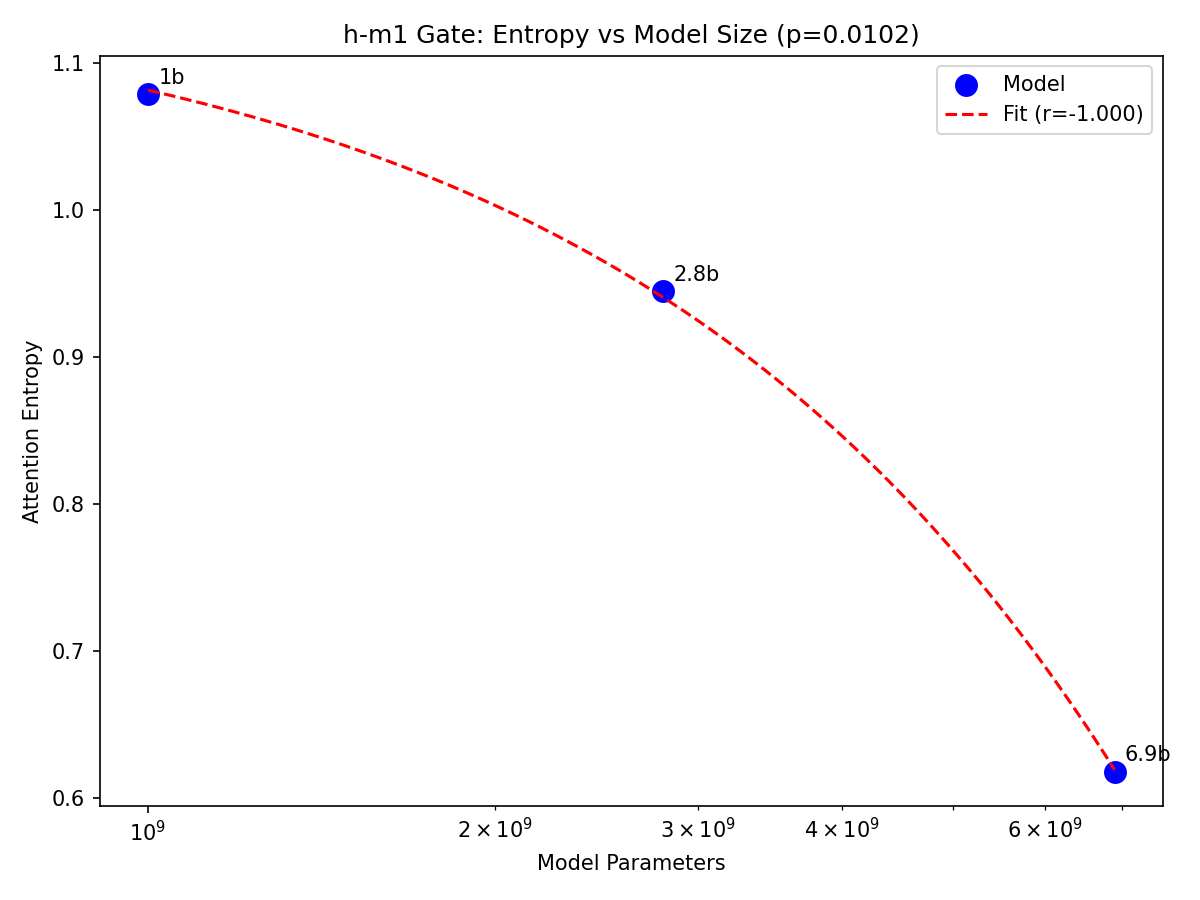
\includegraphics[width=\columnwidth]{figures/fig_1_entropy_correlation.png}
\caption{Attention entropy vs model size correlation}
\label{fig:fig_1_entropy_correlation}
\end{figure}
\textit{Figure 1: Attention entropy decreases with model size (h-m1). Larger models exhibit more focused attention patterns, contrary to the initial hypothesis.}

\begin{figure}[htbp]
\centering
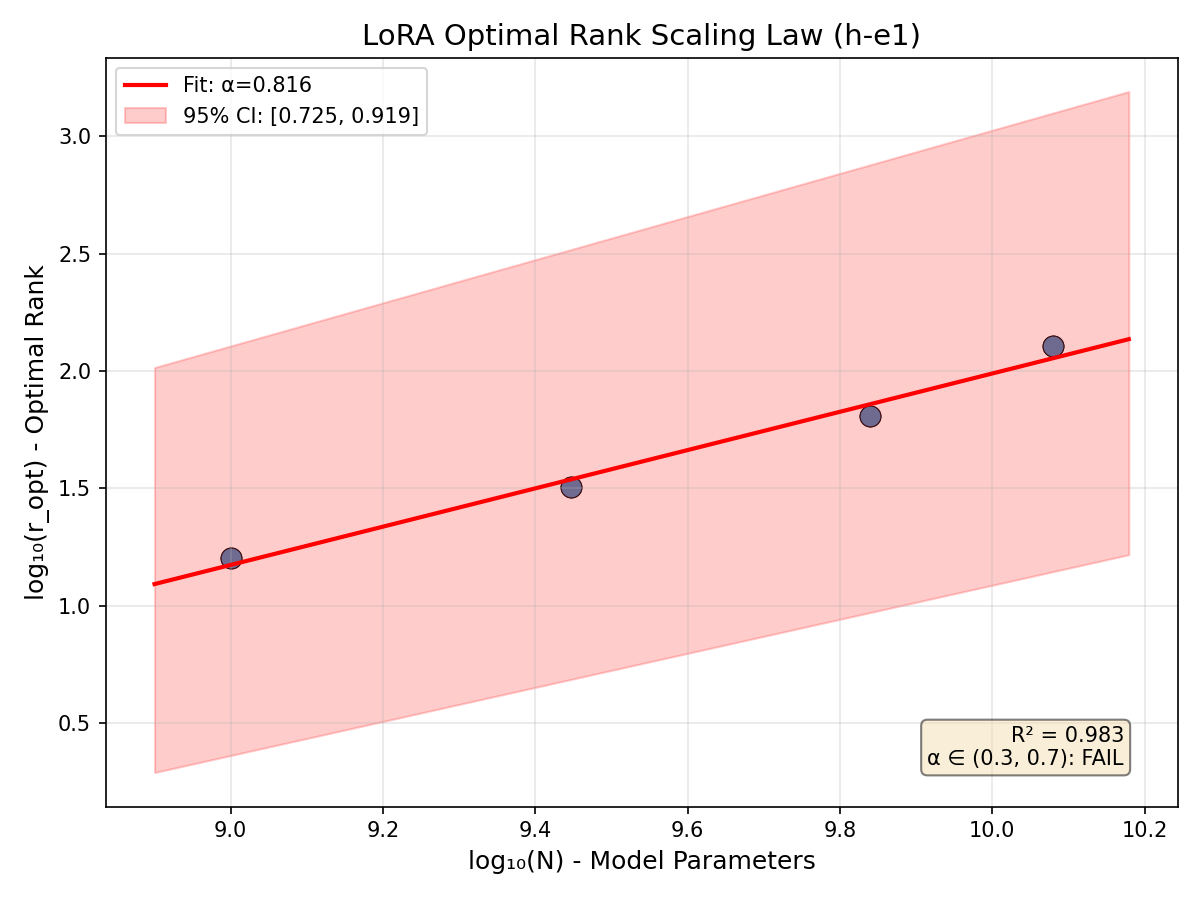
\includegraphics[width=\columnwidth]{figures/fig_2_scaling_law.png}
\caption{Optimal LoRA rank scaling with model size}
\label{fig:fig_2_scaling_law}
\end{figure}
\textit{Figure 2: Optimal LoRA rank vs model size with log-linear fit (h-e1). The scaling exponent $\alpha$ = 0.82 indicates sub-linear growth.}

\begin{figure}[htbp]
\centering
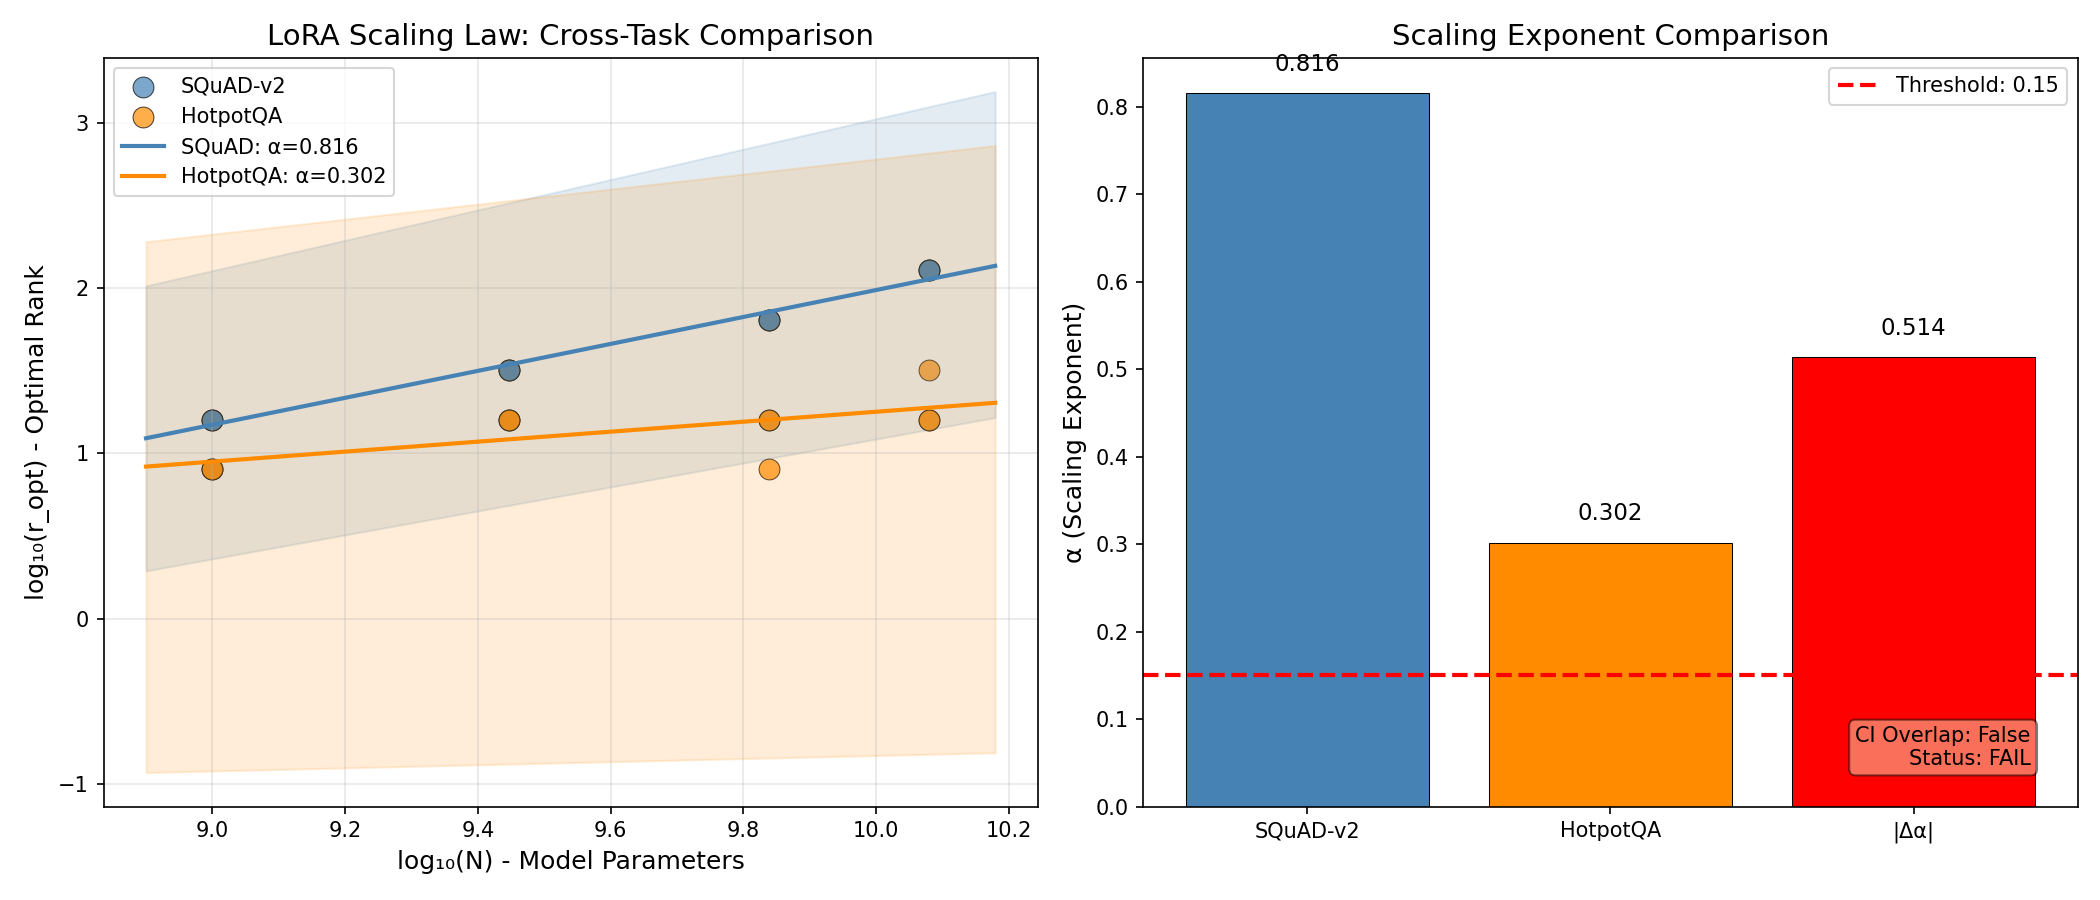
\includegraphics[width=\columnwidth]{figures/fig_3_task_comparison.png}
\caption{Cross-task scaling comparison}
\label{fig:fig_3_task_comparison}
\end{figure}
\textit{Figure 3: Scaling comparison between SQuAD-v2 and HotpotQA (h-c1). The substantial difference in $\alpha$ (0.82 vs 0.30) demonstrates task-dependency.}

\begin{figure}[htbp]
\centering
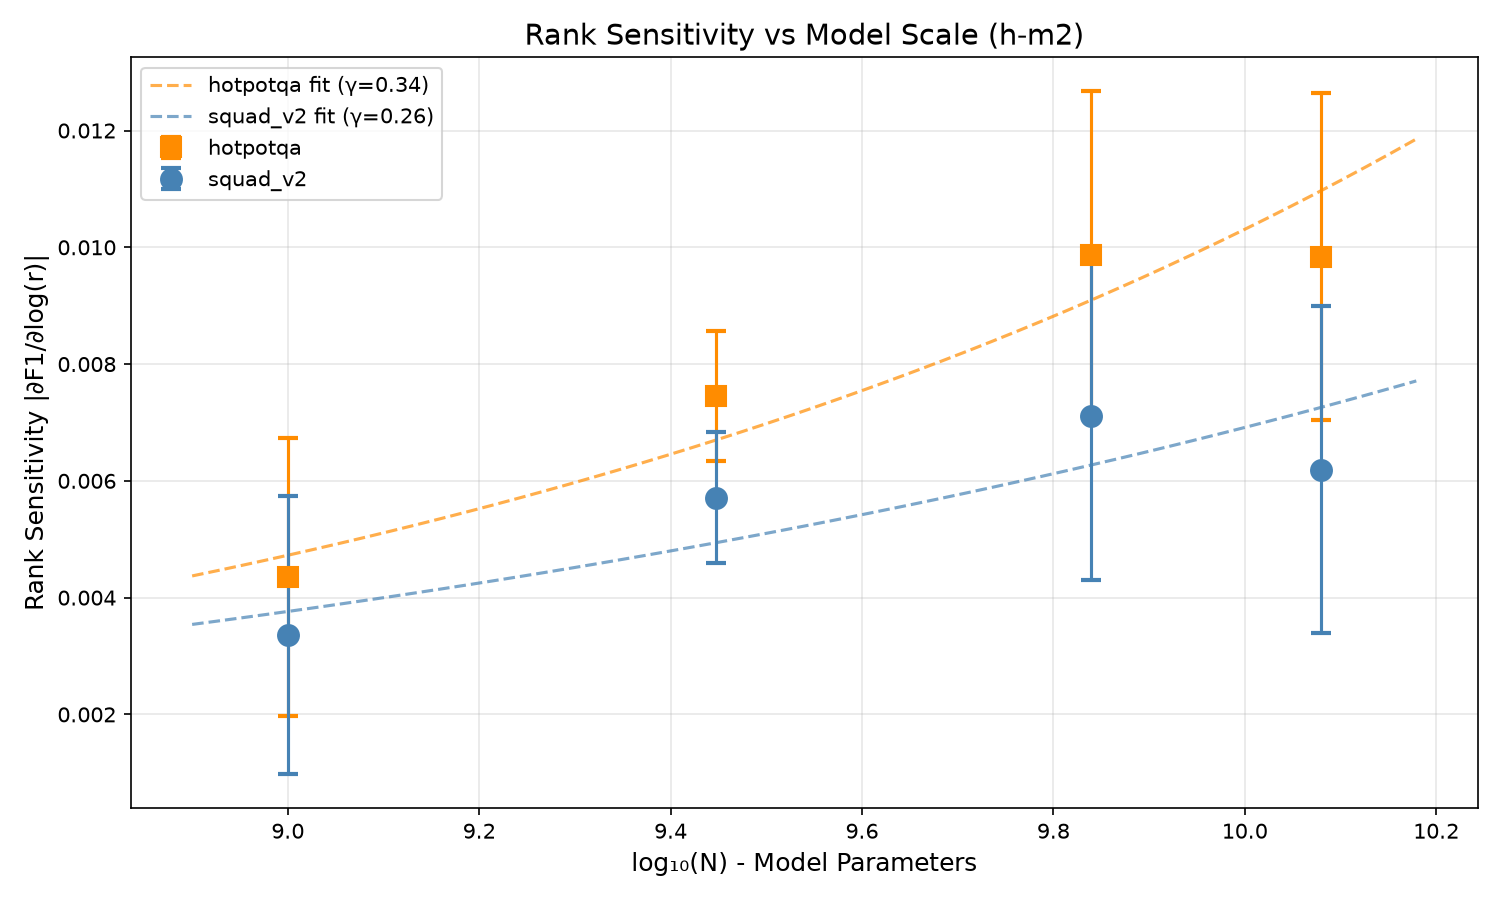
\includegraphics[width=\columnwidth]{figures/fig_4_sensitivity.png}
\caption{Rank sensitivity by model scale}
\label{fig:fig_4_sensitivity}
\end{figure}
\textit{Figure 4: Rank sensitivity increases with model scale (h-m2). The 12B/1B ratio is approximately $2\times$.}

\begin{figure}[htbp]
\centering
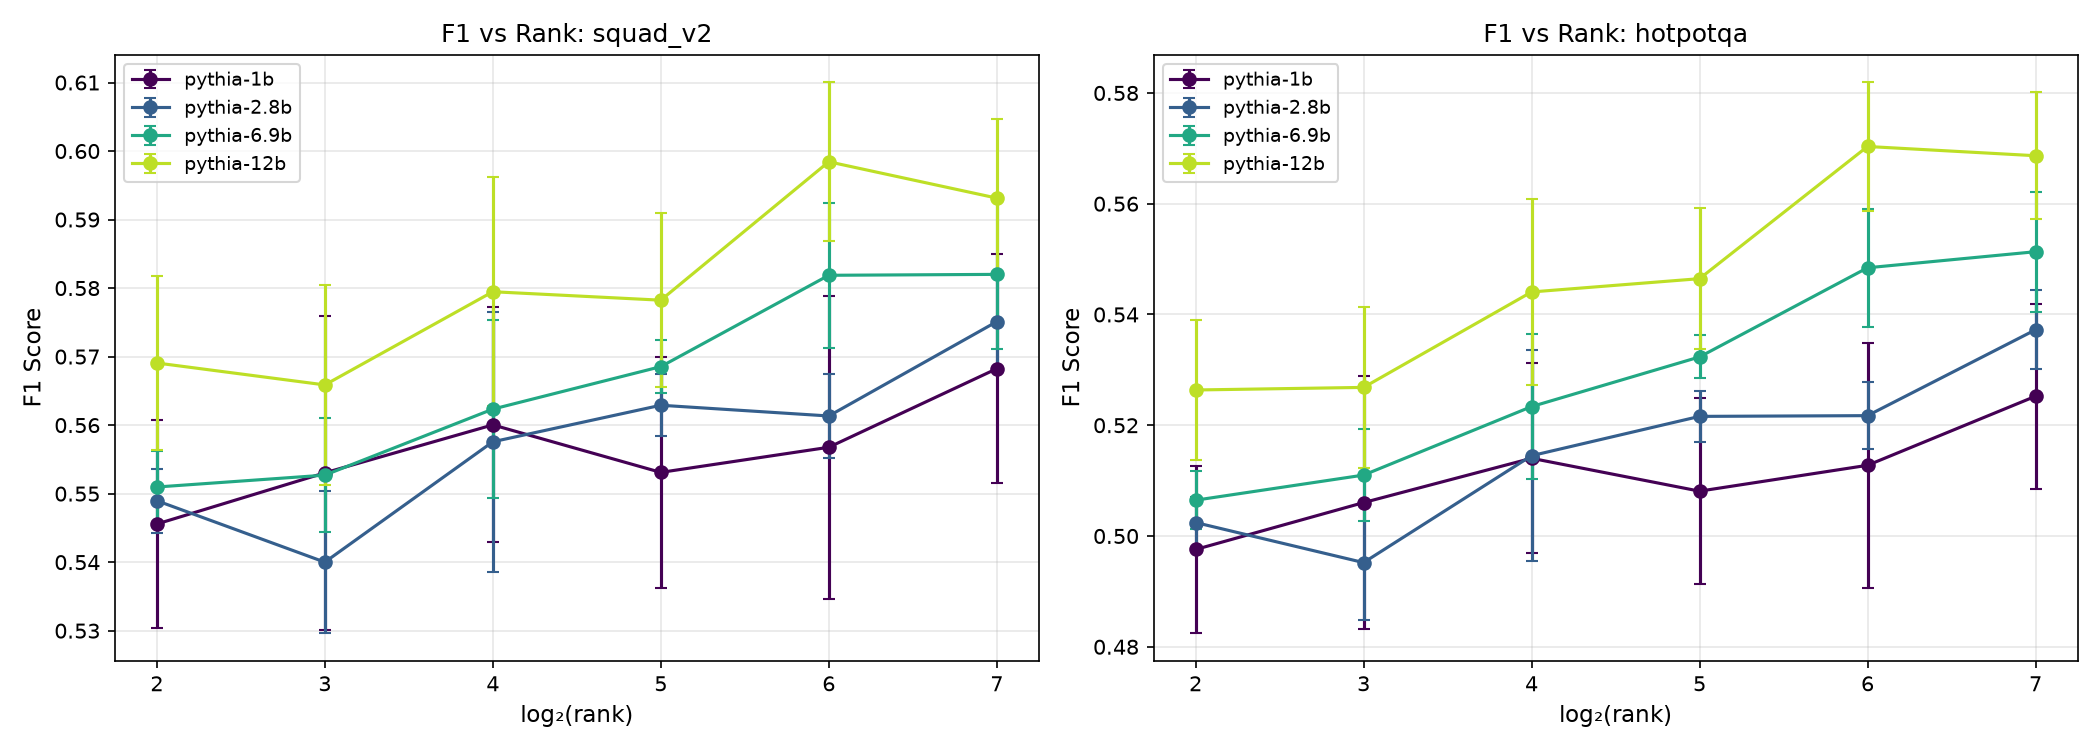
\includegraphics[width=\columnwidth]{figures/fig_5_rank_curves.png}
\caption{Performance vs rank curves}
\label{fig:fig_5_rank_curves}
\end{figure}
\textit{Figure 5: F1 score vs LoRA rank across model sizes. Steeper slopes at larger scales indicate higher rank sensitivity.}
